%
%
%
\section{EXPERIMENTS}

%
%
%
In this section we complement our analysis with performance results of our parallel implementation of the 2D hybridized SBP-SAT problem.
We developed code used to solve this system in C++ and utilize the PETSc library to implement the linear algebra operations utilized throughout. 
All linear systems are solved using the direct LU solver provided by PETSc.
We implemented thread parallel routines in OpenMP \citep{openmp08}, utilizing the parallelism made available through hybridization.
Our code ran on the University of Oregon's Talapas supercomputing cluster on an Intel Xeon E5-2690 v4 CPU. 
Profiling information including cache accesses, writes, and flop counts were sought using the PAPI profiler \citep{jagode2019papi}.

%
%
%
\subsection{Strong scaling}
%
%
%
We ran several problems with an fixed number of grid points in the problem's volume, varying $n$ and $\ell$ proportionally, \emph{i.e.}, $\bar{n} = n \times \ell$ for some fixed $\ell$.
Each hybridized system has more than 705\,600 points as the $\textbf{F}$  factors increase the size of the system as we add elements.
Each problem was run with several thread configurations, from 1 thread to 28 threads. 
Additionally total number of elements varied between 9, with 78\,400 grid points per element and 1600, with 441 grid points per elements. 
With this we have a profile of the problem's strong-scaling performance, as well as an insight in the effects of varying element size within the same problem.  

%
%
%
The optimal runtime was found at $\ell^2 = 100$ for all thread configurations. 
A full table of the compute time separated by thread count and element count is given in \figref{fig:tts_total}.
We plot the speedup \emph{i.e.}, $S = T/T_{p}$ for the number of threads $p$ for the best and worst choices of $\ell$ in \figref{fig:sca_exp_a}.

%
%
%
\begin{figure}[!hb]
	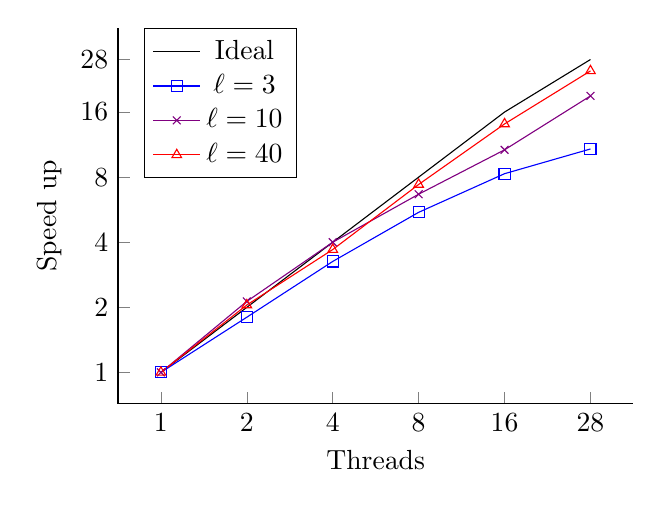
\begin{tikzpicture}
    \begin{axis}[
        legend style = {
            at={(0.05, 1)},
            anchor = north west,
            legend columns = 1},
        height=2.5in,
        width=3.2in,
        axis x line*=bottom,
        axis y line*=left,
        symbolic x coords = {1, 2, 4, 8, 16, 28},
        xtick = {1, 2, 4, 8, 16, 28},
        ytick = {1, 2, 4, 8, 16, 28},
        domain = 1:28,
        range = 1:28,
        ymode = log,
        log ticks with fixed point,
        xlabel={Threads},
        ylabel={Speed up}]      
        \addplot[
            no markers,
            color=black] coordinates {
                (1, 1)
                (2, 2)
                (4, 4)
                (8, 8)
                (16, 16)
                (28, 28)
            };                 
        \addplot[
            mark=square,
            color=blue] coordinates {
                (1, 1)
                (2, 1.8)
                (4, 3.26)
                (8, 5.5)
                (16, 8.3)
                (28, 10.8)
            };
        \addplot[
            mark=x,
            color=violet] coordinates {
                (1, 1)
                (2, 2.13)
                (4, 4)
                (8, 6.67)
                (16, 10.7)
                (28, 19)
            };
        \addplot[
            mark=triangle,
            color=red] coordinates {
                (1, 1)
                (2, 2.05)
                (4, 3.7)
                (8, 7.4)
                (16, 14.1)
                (28, 24.8)
            };
        \addlegendentry{Ideal}
        \addlegendentry{$\ell = 3$}
        \addlegendentry{$\ell = 10$}
        \addlegendentry{$\ell = 40$}
    \end{axis}
\end{tikzpicture}
	\caption{
	    The speed up of three pairs of $n$ and $\ell$ such that $\bar{n}$ is constant. 
	    Scaling improves as $\ell$ increases; however, overall runtime is best at $ell = 10$. 
	    }
    \label{fig:sca_exp_a}
\end{figure}

Here, speedup scaling is proportional to $\ell$. 
This is not in proportion to the overall runtime by choice of $\ell$; the best case ($\ell^2 = 100$) has worse scaling than $\ell^2 = 1600$ and better than $\ell^2 = 9$.
This suggests that different components of the problem are contributing to the performance on either end of of this scale. 

%
%
%
To this end we profiled the runtime of the 7 operations that comprise the hybridized system. 
Two operations utilize the majority of the compute time, those being SpMV from \eqnref{eqn:global_system_b} and MatMul from \eqnref{eqn:global_system_a}.
The remaining 5 operations average $8\%$ of the compute time when run on a single thread. 
The compute time of the two major operations are plotted in \figref{fig:runtime_comps} with the same configuration of problems. 

%
%
%
\begin{figure}
\centering
\begin{subfigure}[b]{1\columnwidth}
\centering
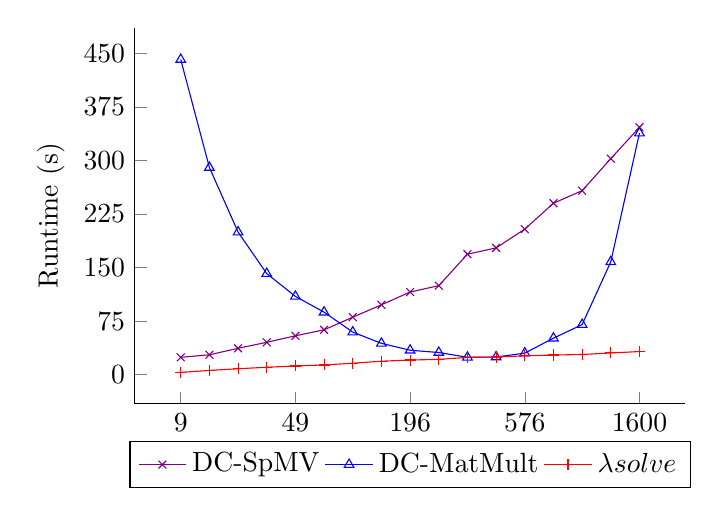
\begin{tikzpicture}
    \begin{axis}[
        legend style={
            at={(0.5,-0.1)},
            anchor=north,legend columns=-1},
        height=2.5in,
        width=3.375in,
        axis x line*=bottom,
        axis y line*=left,
        symbolic x coords = {9, 16, 25, 36, 49, 64, 100, 144, 196, 225, 400, 441, 576, 784, 900, 1225, 1600},
        xtick = {9, 49, 196, 576, 1600},
        ytick distance=75,
        domain = 9:1600,
        range = 0:450,
        xlabel={Elements},
        ylabel={Runtime (s)}]
        \addplot[
            mark=x,
            color=violet] coordinates {
                (9, 24.325156)
            	(16, 27.834308) 
            	(25, 36.956056)
            	(36, 45.347331)
            	(49, 54.437361)
            	(64, 62.814148)
            	(100, 80.488467)
            	(144, 97.845769)             	 
            	(196, 115.743751) 
            	(225, 124.628909) 
            	(400, 168.691478) 
            	(441, 177.584231) 
            	(576, 203.812683) 
            	(784, 240.088173) 
            	(900, 257.634123) 
            	(1225, 302.521926)
            	(1600, 346.441605)		
            };                
        \addplot[
            mark=triangle,
            color=blue] coordinates {
                (9, 441.321048)
            	(16, 290.10575)
            	(25, 199.676772)
            	(36, 141.542836)
            	(49, 109.624197)
            	(64, 87.516978)
            	(100, 59.597739)
            	(144, 43.86835)             	 
            	(196, 34.223977) 
            	(225, 31.043727) 
            	(400, 24.364813) 
            	(441, 24.756918) 
            	(576, 30.185676) 
            	(784, 51.117228) 
            	(900, 70.110809) 
            	(1225, 158.006306)
            	(1600, 338.225247)		
            };
        \addplot[
            mark=+,
            color=red] coordinates {
                (9, 3.186158)
            	(16, 5.987428)
            	(25, 8.304203)
            	(36, 10.420171)
            	(49, 12.213909)
            	(64, 13.637598)
            	(100, 16.047212)
            	(144, 18.873235)             	 
            	(196, 20.515413) 
            	(225, 21.414372)
            	(400, 24.244844) 
            	(441, 24.780033) 
            	(576, 26.379761) 
            	(784, 27.517695) 
            	(900, 28.265589) 
            	(1225, 30.447891)
            	(1600, 32.383344)		
            };
        \addlegendentry{DC-SpMV}
        \addlegendentry{DC-MatMult}
        \addlegendentry{$\symbf{\lambda} \text{ solve}$} 
    \end{axis}
\end{tikzpicture}
\end{subfigure}
\begin{subfigure}[b]{1\columnwidth}
\centering
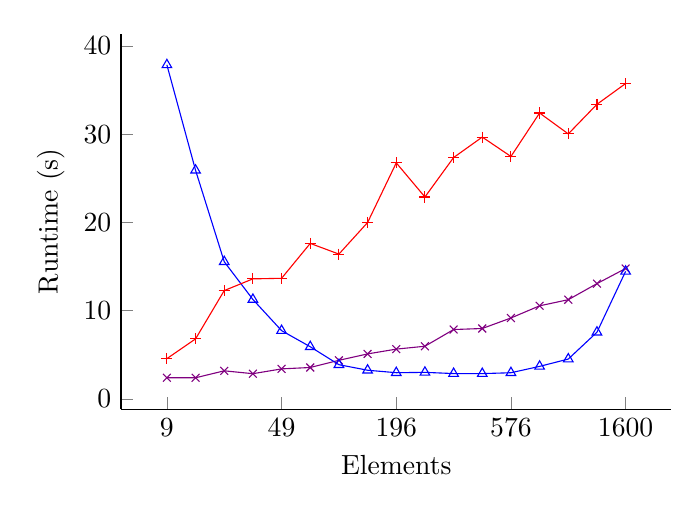
\begin{tikzpicture}
    \begin{axis}[
        height=2.5in,
        width=3.375in,
        axis x line*=bottom,
        axis y line*=left,
        symbolic x coords = {9, 16, 25, 36, 49, 64, 100, 144, 196, 225, 400, 441, 576, 784, 900, 1225, 1600},
        xtick = {9, 49, 196, 576, 1600},
        ytick distance=10,
        domain = 9:1600,
        range = 0:40,
        xlabel={Elements},
        ylabel={Runtime (s)}]
        \addplot[
            mark=x,
            color=violet] coordinates {
                (9, 2.397702)
                (16, 2.394517) 
                (25, 3.180994)
                (36, 2.855465)
                (49, 3.40153)
                (64, 3.558418)
                (100, 4.372501)
                (144, 5.095191)                  
                (196, 5.641578) 
                (225, 5.964769) 
                (400, 7.857667) 
                (441, 7.976037) 
                (576, 9.166833) 
                (784, 10.545802) 
                (900, 11.238055) 
                (1225, 13.058728)
                (1600, 14.773929)       
            };                            
        \addplot[
            mark=triangle,
            color=blue] coordinates {
                (9, 37.839475)
                (16, 25.899214)
                (25, 15.539969)
                (36, 11.263805)
                (49, 7.735455)
                (64, 5.908895)
                (100, 3.875921)
                (144, 3.248426)                  
                (196, 2.967249) 
                (225, 3.007436) 
                (400, 2.871237) 
                (441, 2.866318) 
                (576, 2.963138) 
                (784, 3.684828) 
                (900, 4.5139599) 
                (1225, 7.553876)
                (1600, 14.450906)       
            };     
        \addplot[
            mark=+,
            color=red] coordinates {
                (9, 4.562236)
                (16, 6.799783)
                (25, 12.272318)
                (36, 13.599193)
                (49, 13.662346)
                (64, 17.617201)
                (100, 16.404489)
                (144, 19.981687)                 
                (196, 26.740117) 
                (225, 22.875268)
                (400, 27.343023) 
                (441, 29.659641) 
                (576, 27.462272) 
                (784, 32.388184) 
                (900, 30.020221) 
                (1225, 33.37332)
                (1600, 35.725706)       
            };

    \end{axis}
\end{tikzpicture}
\end{subfigure}
\caption{Runtime of routines that significantly contribute to the overall
    runtime for various element configurations. 1 thread (top) and 28 
    threads (bottom). }
\end{figure}

%
%
%
We exclude the time spent factorizing $\textbf{M}$ and $\symbf{\lambda}_{\textbf{A}}$ for this problem, its practical application would likely involve the reuse of these factorization several times. 
It is worth noting that the cost of LU factorization for $\symbf{\lambda}_{\textbf{A}}$ becomes considerable as $\ell^2$ increases. 
This is expected by \eqnref{eqn:lamsize} as the size of $\symbf{\lambda}_{\textbf{A}}$ increases with $\ell$ and by \eqnref{eqn:nz_sum} as the number of non-zeros increases with $\ell$.

%
%
%
\subsection{MatMul analysis}

%
%
%
\begin{figure}[!b]
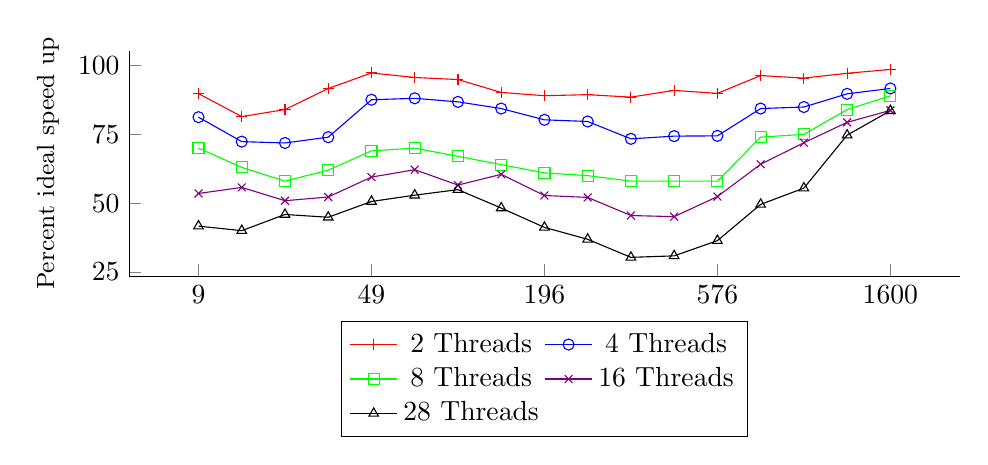
\begin{tikzpicture}
    \begin{axis}[
	    legend style={
            at={(0.5,-0.2)},
            anchor=north,
            legend columns=2},
        height=1.75in,
        width=\columnwidth,
        axis x line*=bottom,
        axis y line*=left,
        symbolic x coords = {9, 16, 25, 36, 49, 64, 100, 144, 196, 225, 400, 441, 576, 784, 900, 1225, 1600},
        xtick = {9, 49, 196, 576, 1600},
        ytick distance=25.,
        domain = 9:1600,
        range = 0:1,
        xlabel={\small Elements ($\ell^2$)},
        ylabel={\small Percent ideal speed up}]
	\addplot[
        mark=+,
        color=red] coordinates { 
            (9,89.80772783)
			(16,81.44809896)
			(25,84.01265431)
			(36,91.65362266)
			(49,97.3178835)
			(64,95.66418795)
			(100,94.91731162)
			(144,90.23017479)
			(196,89.04560603)
			(225,89.42606936)
			(400,88.52873523)
			(441,90.96957938)
			(576,89.89312948)
			(784,96.362808)
			(900,95.4433221)
			(1225,97.19841906)
			(1600,98.58183248)};
	\addlegendentry{2 Threads}
    \addplot[
        mark=o,
        color=blue] coordinates {
            (9,81.24280595)
			(16,72.35409511)
			(25,71.87422205)
			(36,73.97099956)
			(49,87.57828937)
			(64,88.09522093)
			(100,86.80642458)
			(144,84.38193744)
			(196,80.28113664)
			(225,79.68067235)
			(400,73.36438178)
			(441,74.36115039)
			(576,74.44781356)
			(784,84.37458405)
			(900,84.94134329)
			(1225,89.72037773)
			(1600,91.68107848)};
	\addlegendentry{4 Threads}
	\addplot[
        mark=square,
        color=green] coordinates {
            (9,70)
			(16,63)
			(25,58)
			(36,62)
			(49,69)
			(64,70)
			(100,67)
			(144,64)
			(196,61)
			(225,60)
			(400,58)
			(441,58)
			(576,58)
			(784,74)
			(900,75)
			(1225,84)
			(1600,89)};
	\addlegendentry{8 Threads}
	\addplot[
        mark=x,
        color=violet] coordinates {
            (9,53.52149343)
			(16,55.72203392)
			(25,50.88135743)
			(36,52.24498021)
			(49,59.47561476)
			(64,62.16044819)
			(100,56.57392172)
			(144,60.4699287)
			(196,52.77826458)
			(225,52.08890179)
			(400,45.50386094)
			(441,45.10367777)
			(576,52.38086479)
			(784,64.13954692)
			(900,71.95346234)
			(1225,79.35939415)
			(1600,83.71552989)};
	\addlegendentry{16 Threads}			
	\addplot[
        mark=triangle,
        color=black] coordinates {
            (9,41.65350074)
			(16,40.00476479)
			(25,45.89013843)
			(36,44.87916193)
			(49,50.6130524)
			(64,52.89663054)
			(100,54.91573947)
			(144,48.23033634)
			(196,41.1925286)
			(225,36.86544072)
			(400,30.30651572)
			(441,30.84708825)
			(576,36.38237089)
			(784,49.5441113)
			(900,55.47142684)
			(1225,74.70446109)
			(1600,83.58972861)};
	\addlegendentry{28 Threads}
    \end{axis}
\end{tikzpicture}
\caption{Performance of the decomposed MatMult kernel on a fixed problem size (705600 grid points) for various thread counts and total elements.}
\end{figure}
										
													


%
%
%
Out of the two kernels that comprise the majority of the runtime we see the most variability in MatMul operation from \eqnref{eqn:global_system_a}. 
The operation is implemented in a similar manner to batched general matrix multiply (GEMM) methods \citep{wei2022lbbgemm}, but as our intermediate results from $\textbf{M}^{-1}\textbf{F}$ are dense vectors we instead compute a batched vector inner product. Batching methods allocate single threads to self-contained operations in contrast to  of coordinating multiple threads to solve a larger problem. 

These results show an optimal range of elements to minimize runtime between 100 to 600 elements for $\bar{n} = 840$.
When there are too few elements the problem has a greater number of FLOPs and bytes loaded. 
The total FLOPs of this operation decrease for MatMul at a rate of $1/\ell^4$ from \eqnref{eqn:flops_fmf} and the total bytes decrease at $1/\ell^3$ from \eqnref{eqn:bytes_fmf}.
As both of these terms decrease, our runtime decreases proportionally until we reach approximately 600 elements. 

%The increase in runtime at this point is associated with increasing number of non-zeros in $\symbf{\lambda}_{\textbf{A}}$. 

\begin{figure}
	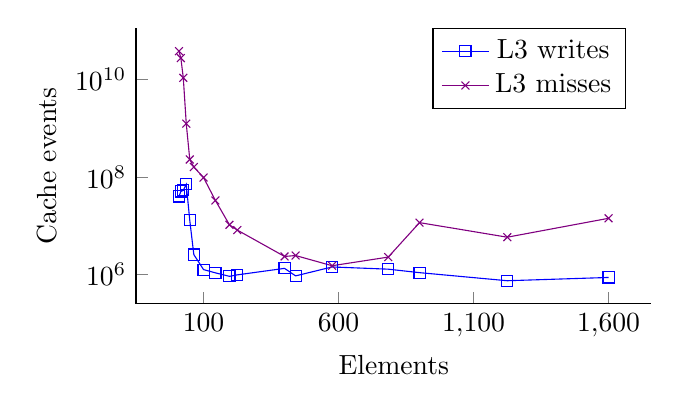
\begin{tikzpicture}
    \begin{axis}[
        legend style = {
            at={(0.95, 1)},
            anchor = north east,
            legend columns = 1},
        height=2in,
        width=3.2in,
        axis x line*=bottom,
        axis y line*=left,
        xtick={100, 600, 1100, 1600},
        domain = 1:1600,
        range = 1:1e10,
        ymode = log,
        xlabel={Elements},
        ylabel={Cache events}]                     
        \addplot[
            mark=square,
            color=blue] coordinates {
                (9,40205717)
                (16,50879473)
                (25,53610700)
                (36,71074406)
                (49,12977133)
                (64,2579077)
                (100,1268591)
                (144,1087212)
                (196,922253)
                (225,988667)
                (400,1344455)
                (441,941907)
                (576,1436403)
                (784,1294177)
                (900,1097877)
                (1225,749441)
                (1600,874811)
            };
        \addplot[
            mark=x,
            color=violet] coordinates {
                (9,38402769309)
                (16,27712437645)
                (25,10922310284)
                (36,1249621355)
                (49,230572757)
                (64,161468223)
                (100,98065404)
                (144,33179551)
                (196,10523799)
                (225,8202903)
                (400,2360980)
                (441,2462776)
                (576,1522457)
                (784,2288844)
                (900,11663667)
                (1225,5858703)
                (1600,14307506)
            };
        \addlegendentry{L3 writes}
        \addlegendentry{L3 misses}
    \end{axis}
\end{tikzpicture} 
	\caption{L3 writes and misses profiled for the strong scaling problem configuration. 
	Though the total bytes written out to $\symbf{\lambda}_{\textbf{A}}$ increase with additional elements, fewer occur with every batch. 
	Fewer writes per batch to more rows of $\symbf{\lambda}_{\textbf{A}}$ increase our cache misses and overall runtime.
	}
	\label{fig:mmwm}
\end{figure}

%but writes increase with the rate of non-zeros in $\symbf{\lambda}_{\textbf{A}}$ in \eqnref{eqn:nz_sum}. 

%As each element becomes smaller and we increase the number of iterations, the number of writes per iteration decrease. 



%This CPU is rated at a peak single-threaded FLOP rate of 8 GFLOPS/s and a peak memory bandwidth of 86 GB/s.


%From this figure we see that the MatMul operation has a region of optimal performance between 196--576 elements, but begins to perform poorly outside of this range. 
%This is clear as \fig



\subsection{SpMV analysis}
The SpMV kernel is similarly batched to compute $\textbf{F}^\intercal \times (\textbf{M}^{-1}_{i} \bar{\textbf{g}})$ for each element. 
Unlike MatMul, each intermediate vector in $\textbf{M}^{-1}_{i} \bar{\textbf{g}}$ is unique since $\bar{\textbf{g}}$ is unique. 
Additionally, we compute proportionally fewer batches of $n^2 \times n$ SpMV than MatMul, and write out to significantly fewer memory locations. 
We still encounter the same write miss penalty as we both increase the size of the intermediate vector $\textbf{F}^\intercal \times (\textbf{M}^{-1}_{i} \bar{\textbf{g}})$ and decrease the size of each batch operation proportionally.
Even at the smallest element size each batch write 21 doubles, which is larger than a typical cache line. 

%
%
%
\subsection{Memory behavior}

%
%
%
To investigate the decreasing performance of our MatMul and SpMV operations we chose pairs of $\bar{n}$ and $\ell$ with similar total flops for the MatMul kernel.
These problems averaged $1.32\mathrm{e}11$ flops with a coefficient of variation of $2.3\mathrm{e}{-3}$.
Though the flops between each problem varies insignificantly, and the bytes loa\-ded \emph{decrease}, the number of entries in $\symbf{\lambda_{\textbf{A}}}$ --- and hence the number of bytes written \emph{increases}. 
This is illustrated in on the left of \figref{fig:mem_exp_b}; this also plots the measured number of L3 cache writes in MatMul kernel on the right. 
The number of L3 writes grows proportional to the number of entries in $\symbf{\lambda_{\textbf{A}}}$.
The number of entries are approximately $80\times$ greater than the number of L3 writes. This is slightly less than the number of 8 byte doubles that fit into a 128 byte cache line.

%
%
%
\begin{figure}[!h]
	\centering
\begin{tikzpicture}
  \begin{groupplot}[group style={
        vertical sep=2.5cm,
        horizontal sep=1.0cm,
        group size=2 by 1},
        width = {0.55\columnwidth},
        height = {0.4\columnwidth},
        xtick = {81, 196, 400},
        axis x line*=bottom,
        axis y line*=left
        ]
     \nextgroupplot[
        legend to name={CommonLegend}, 
            legend style = {
                at={(0.55, 1)},
                anchor = north,
                legend columns = 1}]
    \addplot[mark=o, color=black,
            ytick = {10000000, 20000000},
            ] coordinates {
        (64, 7292200)
        (81, 8332892) 
        (100, 9370368)
        (144, 11413376)
        (196, 13484800)
        (400, 19672672)};
    \nextgroupplot[]
    \addplot[mark=square, only marks,
            ytick = {1000000, 2000000},
            ] coordinates {
        (64, 726220)
        (81, 820642) 
        (100, 981485)
        (144, 1090082)
        (196, 1480461)
        (400, 2068669)};
    \end{groupplot}
    \node[anchor=south, rotate=90] (title-y) at ($(group c1r1.west)-(0.55,0cm)$) {\small Entries in $\symbf{\lambda_{\textbf{A}}}$};
    \node[anchor=south, rotate=90] (title-y) at ($(group c2r1.west)-(0.45,0cm)$) {\small L3 writes to $\symbf{\lambda_{\textbf{A}}}$};
    \node[anchor=north] (title-x) at ($(group c1r1.south)-(0,0.5cm)$) {\small Elements ($\ell^2$)};
    \node[anchor=north] (title-x) at ($(group c2r1.south)-(0,0.5cm)$) {\small Elements ($\ell^2$)};
\end{tikzpicture}
	\caption{
	    The amount of non-zero elements in $\symbf{\lambda_{\textbf{A}}}$ for a set of problems with similar flop profiles (left) and the number of L3 cache data writes measured with PAPI (right). 
	    While the total flops are similar, the size and number of entries in $\symbf{\lambda_{\textbf{A}}}$ continues to grow. 
	    }
    \label{fig:mem_exp_b}
\end{figure}

\noindent
The runtime of MatMul SpMV, and the LU factorization of $\symbf{\lambda}_{\textbf{A}}$ all increase in runtime, even though the flops remaining minimally changed and the bytes loaded decrease. 
We illustrate this in \figref{fig:mem_exp_a}. 
The growth of the $\symbf{\lambda}_{\textbf{A}}$ factorization ide to the additional non-zero entries increasing its complexity.
For the other two operations this suggests that the greatest impact to runtime at this scale is the number of writes to $\symbf{\lambda}_{\textbf{A}}$, \emph{i.e.}, that these operations are becoming write bound.
This is affirmed by \figref{fig:mmwm}, as additional the sum of L3 write and misses in the MatMul kernel as we increase the number of elements while fixing grid points.  


\begin{figure}[h]
	\centering
\begin{tikzpicture}
  \begin{groupplot}[group style={
        vertical sep=0.6cm,
        horizontal sep=0.6cm,
        group size=2 by 2},
        width = {0.55\columnwidth},
        height = {0.4\columnwidth},
        xtick = {81, 196, 400},
        axis x line*=bottom,
        axis y line*=left
        ]
    \nextgroupplot[
        legend to name={CommonLegend}, 
            legend style = {
                at={(0.55, 1)},
                anchor = north,
                legend columns = 1}]
    \addplot[mark=triangle,
            color=blue,
            ytick = {0, 15, 30},
            ] coordinates {
        (64, 2.850768)
        (81, 3.575837) 
        (100, 4.804298)
        (144, 7.409625)
        (196, 10.974236)
        (400, 25.562375)};
    \addlegendentry{SpMV}
    \addlegendimage{mark=x, color=violet}
    \addlegendentry{MatMul}
    \addlegendimage{mark=+, color=red}
    \addlegendentry{$\symbf{\lambda} \text{ factorize}$}
    \nextgroupplot[]
    \addplot[mark=x,
            color=violet] coordinates {
        (64, 4.088154)
        (81, 4.365303) 
        (100, 4.467857)
        (144, 4.938318)
        (196, 5.806286)
        (400, 7.537781)};
    \nextgroupplot
    \addplot[mark=+,
            color=red] coordinates {
        (64, 13.426294)
        (81, 16.718145) 
        (100, 20.588018)
        (144, 31.325170)
        (196, 41.698411)
        (400, 82.765920)};
    \end{groupplot}
    \node[anchor=north] (title-x) at ($(group c1r2.south)-(0,0.5cm)$) {\small Elements ($\ell^2$)};
    \node[anchor=south, rotate=90] (title-y) at ($(group c1r1.south west)!0.5!(group c1r2.north west)-(0.55,0cm)$) {\small Runtime (s)};
    \node[anchor=west] at ($(group c1r2.east)+(0.75cm,-0.25cm)$) {\ref{CommonLegend}};
\end{tikzpicture}
	\caption{
	    The runtime of three expensive operations using 28 threads on several problem sizes with a similar total flops. 
	    Though the total flops remain essentially the same, the runtime increases for all three kernels.
	    }
	\label{fig:mem_exp_a}
\end{figure}



%
%
%



%\begin{mcfigure}
%	\centering
%	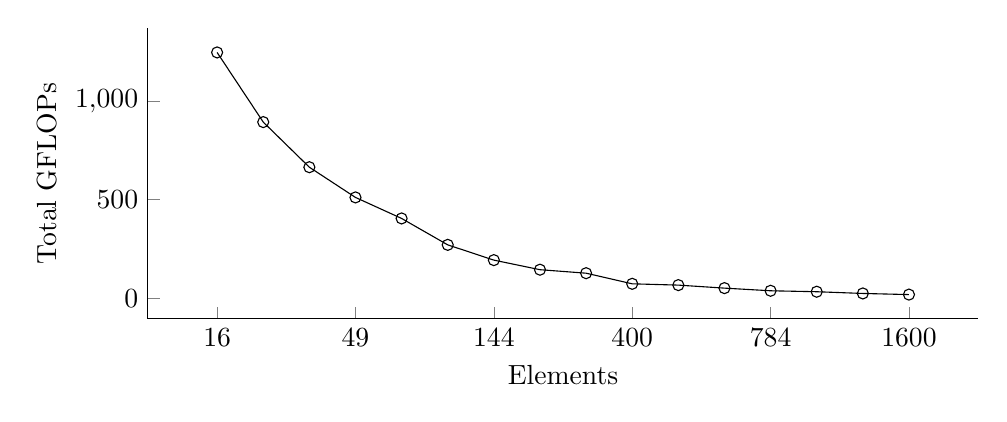
\begin{tikzpicture}
    \begin{axis}[
        height=15em,
        width=\linewidth,
        axis x line*=bottom,
        axis y line*=left,
        symbolic x coords = {16, 25, 36, 49, 64, 100, 144, 196, 225, 400, 441, 576, 784, 900, 1225, 1600},
        xtick = {16, 49, 144, 400, 784, 1600},
        ytick = {0, 500, 1000, 1500},
        domain = 16:1600,
        range = 0:1500,
        xlabel={Elements},
        ylabel={Total GFLOPs}]
        \addplot[
            mark=o,
            color=black] coordinates {
            	(16, 1244.6784)
            	(25, 892.1854771)
            	(36, 663.82848)
            	(49, 510.93504)
            	(64, 404.52048)
            	(100, 270.8420198)
            	(144, 193.61664)             	 
            	(196, 145.152) 
            	(225, 127.4550682) 
            	(400, 73.68496128) 
            	(441, 67.09248) 
            	(576, 51.8616) 
            	(784, 38.46528) 
            	(900, 33.63397632) 
            	(1225, 24.89647104)
            	(1600, 19.16804736)		
            };
    \end{axis}
\end{tikzpicture}

            

%	\captionof{figure}{Total FLOPs used to compute the factorized matrix multiplication in $\textbf{F}^{\intercal} \times (\textbf{M}^{-1} \textbf{F})$ over the number of elements for a constant problem size, $N = 705\kern 0.25em 600$. FLOPs decrease as the size of the constituent inner products decrease in relation to the size of each element.}
%\end{mcfigure}



%\subsection{Delta Solve Analysis}

%\begin{mcfigure}
%	\centering
%	\begin{tikzpicture}
    \begin{axis}[
        height=2.5in,
        width=3.375in,
        axis x line*=bottom,
        axis y line*=left,
        symbolic x coords = {49, 64, 100, 144, 196, 225, 400, 441, 576, 784, 900, 1225, 1600},
        xtick = {49, 144, 400, 784, 1600},
        ytick distance=20,
        domain = 49:1600,
        range = 0:60,
        xlabel={Elements},
        ylabel={Runtime (s)}]
        \addplot[dashed, 
            mark=x,
            color=violet] coordinates {
            	(49, 58.048654)
            	(64, 44.608081)
            	(100, 30.117423)
            	(144, 22.058077)             	 
            	(196, 16.56574) 
            	(225, 14.797055) 
            	(400, 9.426228) 
            	(441, 8.84558) 
            	(576, 7.915462) 
            	(784, 8.569443) 
            	(900, 9.894469) 
            	(1225, 16.662268)
            	(1600, 32.297395)		
            };                                      
        \addplot[dashed, 
            mark=triangle,
            color=blue] coordinates {
            	(49, 7.159366)
            	(64, 7.466476)
            	(100, 8.700982)
            	(144, 10.472512)             	 
            	(196, 11.721377) 
            	(225, 11.966759) 
            	(400, 14.197423) 
            	(441, 14.494765) 
            	(576, 14.587827) 
            	(784, 15.465336) 
            	(900, 15.557051) 
            	(1225, 16.686761)
            	(1600, 19.131444)		
            };
        \addplot[dashed, 
            mark=+,
            color=red] coordinates {
            	(49, 3.739837)
            	(64, 4.359711)
            	(100, 5.000516)
            	(144, 6.416801)             	 
            	(196, 8.051781) 
            	(225, 9.404944)
            	(400, 9.965406) 
            	(441, 13.815412) 
            	(576, 16.399836) 
            	(784, 19.31444) 
            	(900, 20.800298) 
            	(1225, 24.993118)
            	(1600, 29.029143)		
            };

        \addplot[
            mark=o,
            color=black] coordinates {
                (49, 69.749697)
                (64, 57.215341)
                (100, 45.317181)
                (144, 40.655649)             
                (196, 37.752682)
                (225, 36.783105)
                (400, 37.477622)
                (441, 37.671921)
                (576, 38.931754)
                (784, 43.377669)
                (900, 46.279928)
                (1225, 58.368563)
                (1600, 80.487622)
            };

        \addlegendentry{$\textbf{F}^{\intercal} \textbf{M}^{-1} \textbf{F}$}
        \addlegendentry{Style 2}
        \addlegendentry{$\lambda_A \lambda_b$}
        \addlegendentry{Total TTS}

    \end{axis}
\end{tikzpicture}
%\end{mcfigure}

